\section{Sprint planning}
After assembling all the tools in Sprint0, we decided to start with the implementation.
As our understanding of task improved, we were able to come up with user stories from the perspective of user, customer, developer and student.
All user-stories were given to the customer so they can be prioritized. 
All but user-stories concerning our student obligations, like writing project plan, minutes, meetings with supervisor and attending lectures.
Those were mandatory and already added as user-stories of sprint1.
On Monday 02.09.2013. we had the meeting with a customer where we estimated time we need for every user story.
The result of that meeting was the list of the rest of the user-stories for sprin1.
All user stories for finishing our first prototype were on the sprint1 list so we also agreed date for presentation and showing the running demo - Thursday 12.09.2013. 
After that ,at a group meeting, we decoupled user-stories into tasks and we were ready to start with the imlementation.


\subsecion {Sprint1 User-stories}

\section{System Burndown}

\begin{figure}[!t]
	\centering
		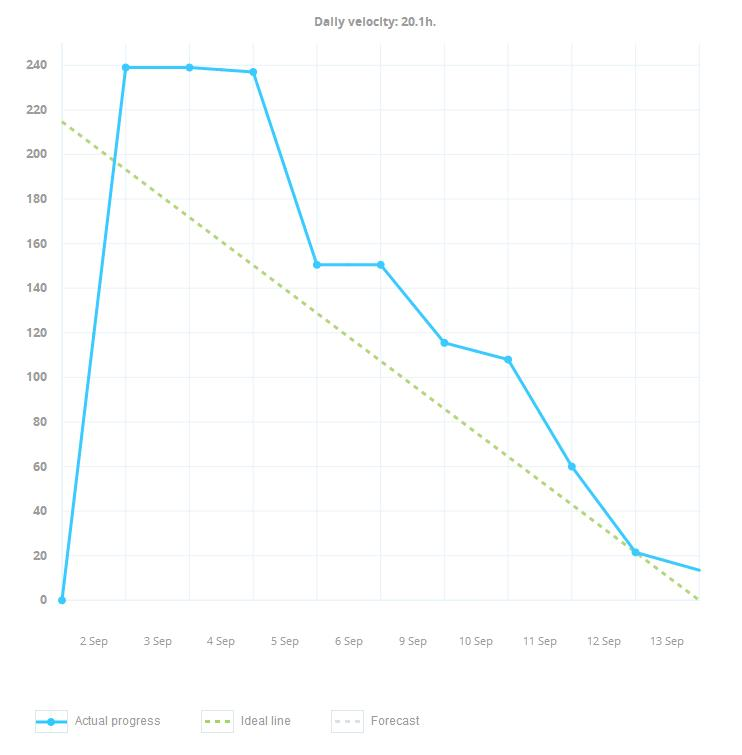
\includegraphics[width=16cm]{burn_down_chart.jpg}
	\caption{Sprint1 Burn Down Chart}
	\label{fig:sprint1_burn_down_chart}
\end{figure}

\section{Architecture}
\section{Implementation}
\section{Testing}
\section{Occurring risks}
\section{Retrospective}
\subsection{Pros}
\subsection{Cons}
\section{Evaluation}